\documentclass[notheorems, handout]{beamer}

\usetheme{Warsaw}
\setbeamertemplate{page number in head/foot}[totalframenumber]
\setbeamertemplate{headline}{}
\setbeamertemplate{navigation symbols}{}
\usefonttheme[onlymath]{serif}

\usepackage[utf8]{inputenc}
\usepackage[T2A]{fontenc}
\usepackage[russian]{babel}

\usepackage{graphicx,subcaption,ragged2e}
\usepackage{tikz}
\usepackage{bm}

\newtheorem{remark}{Замечание}

\title[Статистическое и машинное обучение]{Обучение с учителем}
\institute[Санкт-Петербургский Государственный Университет]{%
	\small
	Санкт-Петербургский государственный университет\\
	Кафедра статистического моделирования
}
\date{16 сентября 2025, Санкт-Петербург}

\begin{document}

\begin{frame}
	\titlepage
\end{frame}

\begin{frame}{Введение}
	\textbf{Машинное обучение}~--- это раздел искусственного интеллекта, в котором разрабатываются методы и алгоритмы, позволяющие компьютерам обнаруживать закономерности в данных и делать прогнозы без явных инструкций.\medskip

	\textbf{Обучение с учителем}~--- один из способов машинного обучения, в ходе которого для каждого примера в обучающем наборе известно, какой результат является правильным.\medskip

	\textbf{Пример задач}:
	\begin{itemize}
		\item Регрессия: предсказание стоимости недвижимости, количества продаж некоторого товара, погоды.
		\item Классификация: предсказание ценовой категории товара, типа изображения, болеет ли человек или нет.
	\end{itemize}
\end{frame}

\begin{frame}{Постановка задачи}
	\textbf{Дано}:
	\begin{enumerate}
		\item Пространство объектов $X$~--- множество описаний объектов (например, фотографии, тексты, таблицы с признаками).
		\item Пространство ответов $Y$~--- множество меток или значений, которые нужно предсказывать (например, классы «кот»/«собака» или числовые значения цен).
		\item Обучающая выборка $D = \{(x_i, y_i)\}_{i=1}^n$, где
		      \begin{itemize}
			      \item $x_i \in X$~--- набор значений признаков (регрессоров).
			      \item $y_i \in Y$~--- целевая переменная или метка, которую мы хотим научиться предсказывать.
			      \item $n$~--- количество индивидов (записей) в выборке.
		      \end{itemize}
	\end{enumerate}

	\textbf{Задача}: построить такую функцию (модель)
	\[
		a:X\longrightarrow Y,
	\]
	чтобы ее предсказания $\hat y=a(x)$ были как можно ближе к истинным ответам $y$.
\end{frame}

\begin{frame}{Функция потерь}
	Чтобы оценить, насколько хорошо модель предсказывает ответы, используется {\bf функция потерь} $L(y, \hat{y})$. Она показывает, насколько велико расхождение между истинными значениями $y$ и его предсказаниями $\hat{y}$.

		{\bf Примеры}:
	\begin{itemize}
		\item Для задачи \textbf{регрессии} наиболее распространенной функцией потерь является среднеквадратичная ошибка (MSE):
		      \[
			      L(y, \hat{y}) = \frac{1}{n}\sum_{i=1}^n (y_i - \hat y_i)^2.
		      \]
		\item Для задачи \textbf{бинарной классификации}, если $\hat y$ представляет собой вектор вероятностей принадлежности к положительному классу, используется кросс-энтропия:
		      \[
			      L(y, \hat{y}) = -\sum_{i=1}^n\left[y_i \ln\hat y_i + (1 - y_i)\ln (1 - \hat y_i)\right].
		      \]
	\end{itemize}
\end{frame}


\begin{frame}{Линейная классификация}
	Пусть целевая переменная $y$ принимает значения $\{-1, 1\}$. Хотим обучить линейную модель так, чтобы плоскость, которую она задает, как можно лучше отделяла объекты одного класса от другого.\medskip

	Линейный классификатор:
	\[
		\hat y=a(x; w)=\operatorname{sign}\langle x, w\rangle.
	\]
	Функция потерь:
	\[
		L(y, \hat{y}) = \sum_{i=1}^{n}\mathbb{I}[y_i \langle x_i, w\rangle < 0] \longrightarrow \min_{w}.
	\]
\end{frame}

\begin{frame}{Линейная классификация. Отступ}
	Величина $M_i=y_i \langle x_i, w\rangle$ называется \textbf{отступом} (margin) классификатора. Абсолютная величина отступа говорит о степени уверенности классификатора.\medskip

	\textbf{Проблема}: функция $\mathbb{I}[M < 0]$ кусочно-постоянная, следовательно функцию потерь невозможно оптимизировать градиентными методами, поскольку во всех точках производная равна нулю.\medskip

	\textbf{Решение}: можно мажорировать эту функцию более гладкой функцией и минимизировать функцию потерь с этой мажорирующей функцией.
\end{frame}

\begin{frame}{Линейная классификация. Функции потерь}
	\begin{enumerate}
		\item Перцептрон: $L(M) = \max(0, -M)$~--- отступы учитываются только для неправильно классифицированных объектах пропорционально величине отступа.
		\item Hinge (SVM): $L(M) = \max(0, 1-M)$~--- объекты, которые классифицированы правильно, но не очень <<уверенно>>, продолжают вносить свой вклад в градиент.
		\item Логистическая: $L(M) = \ln\left(1+e^{-M}\right)$.
	\end{enumerate}
	\begin{figure}
		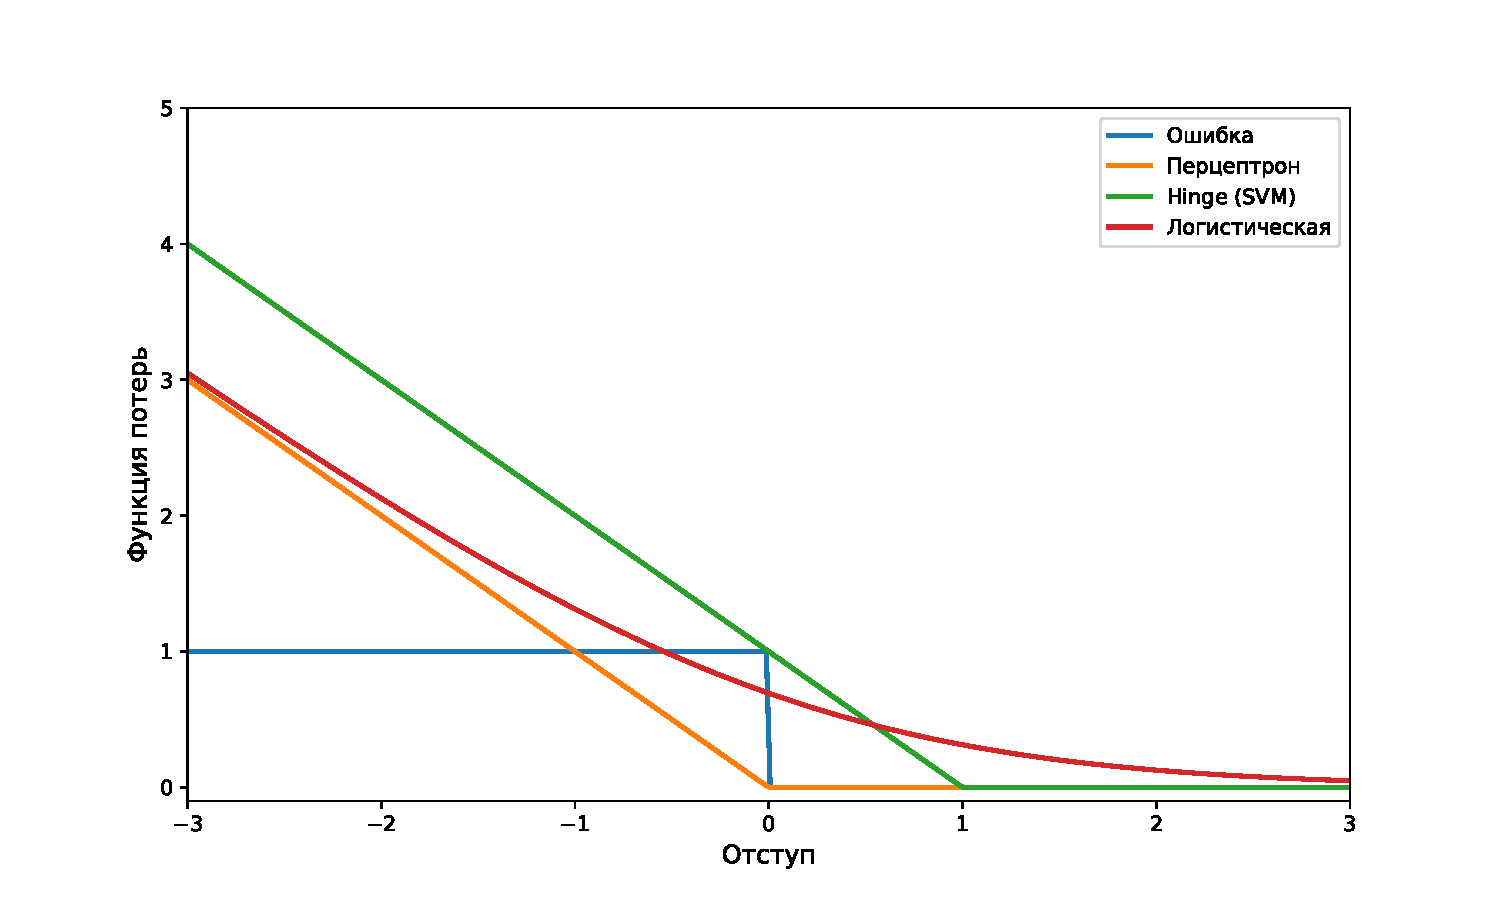
\includegraphics[width=0.75\textwidth]{img/loss_major.pdf}
	\end{figure}
\end{frame}

\begin{frame}{Логистическая регрессия}
	Посмотрим на задачу классификации как на задачу предсказания вероятностей (например, предсказание <<кликабельности>> рекламного баннера).

	\textbf{Принцип работы}: научить линейную модель предсказывать значения $z\in\mathbb{R}$ (логиты), а затем преобразовывать их в вероятности с помощью сигмоиды:
	\[
		z_i=\langle x_i, w\rangle = \ln\frac{p_i}{1 - p_i},\quad p_i = \frac{1}{1+e^{-\langle x_i, w\rangle}}=\sigma(\langle x_i, w\rangle).
	\]
	Функция правдоподобия для распределения Бернулли:
	\[
		p(y~|~\mathbf{X}, w)=\prod_{i=1}^np_i^{y_i}(1-p_i)^{1-y_i}.
	\]
	Прологарифмируем:
	\[
		\sum_{i=1}^n\Big[y_i\ln(\sigma(\langle x_i, w\rangle)) + (1-y_i)\ln(1-\sigma(\langle x_i, w\rangle))\Big].
	\]
\end{frame}

\begin{frame}{Логистическая регрессия. Связь с отступом}
	Теперь пусть $y\in\{-1, 1\}$. Тогда, поскольку $\sigma(z)=1-\sigma(-z)$, логарифм правдоподобия можно представить в следующем виде:
	\begin{align*}
		\ln p (y~|~ \mathbf{X}, w) & = -\sum_{i=1}^n\Big[\mathbb{I}[y_i=1]\sigma(z_i)+\mathbb{I}[y_i=-1]\left(1-\sigma(z_i)\right)\Big] \\
		                           & = -\sum_{i=1}^n \ln\sigma(y_i\langle x_i, w\rangle)                                                \\
		                           & = \sum_{i=1}^n \ln\left(1 + e^{-M}\right)
	\end{align*}

	Таким образом, функцию потерь в логистической регрессии можно представить в виде функции от отступа.
\end{frame}

\end{document}